% fig3_regional_slopes.tex — Slopes Educacionais nas 5 Macro-Regiões
% Compilar standalone via: pdflatex fig3_regional_slopes.tex
\documentclass[border=6pt]{standalone}
\usepackage[T1]{fontenc}
\usepackage[utf8]{inputenc}
\usepackage{amsmath,amssymb}
\usepackage{tikz}
\usetikzlibrary{arrows.meta,calc}

% Paleta Institucional e Okabe-Ito
\definecolor{instblue}{HTML}{012169}
\definecolor{oitoblue}{HTML}{0072B2}
\definecolor{green}{HTML}{009E73}
\definecolor{vermillion}{HTML}{D55E00}
\definecolor{orange}{HTML}{E69F00}
\definecolor{gridgray}{HTML}{E5E5E5}
\definecolor{axisgray}{HTML}{333333}

\begin{document}
% Coordinate map:
% x represents schooling years [3, 17], scale: 1 cm per 1.5 years -> X(x) = (x - 3) * 0.85
% y represents AI exposure [0, 5.5], scale: 1 cm per 1.0 unit -> Y(y) = y * 1.3
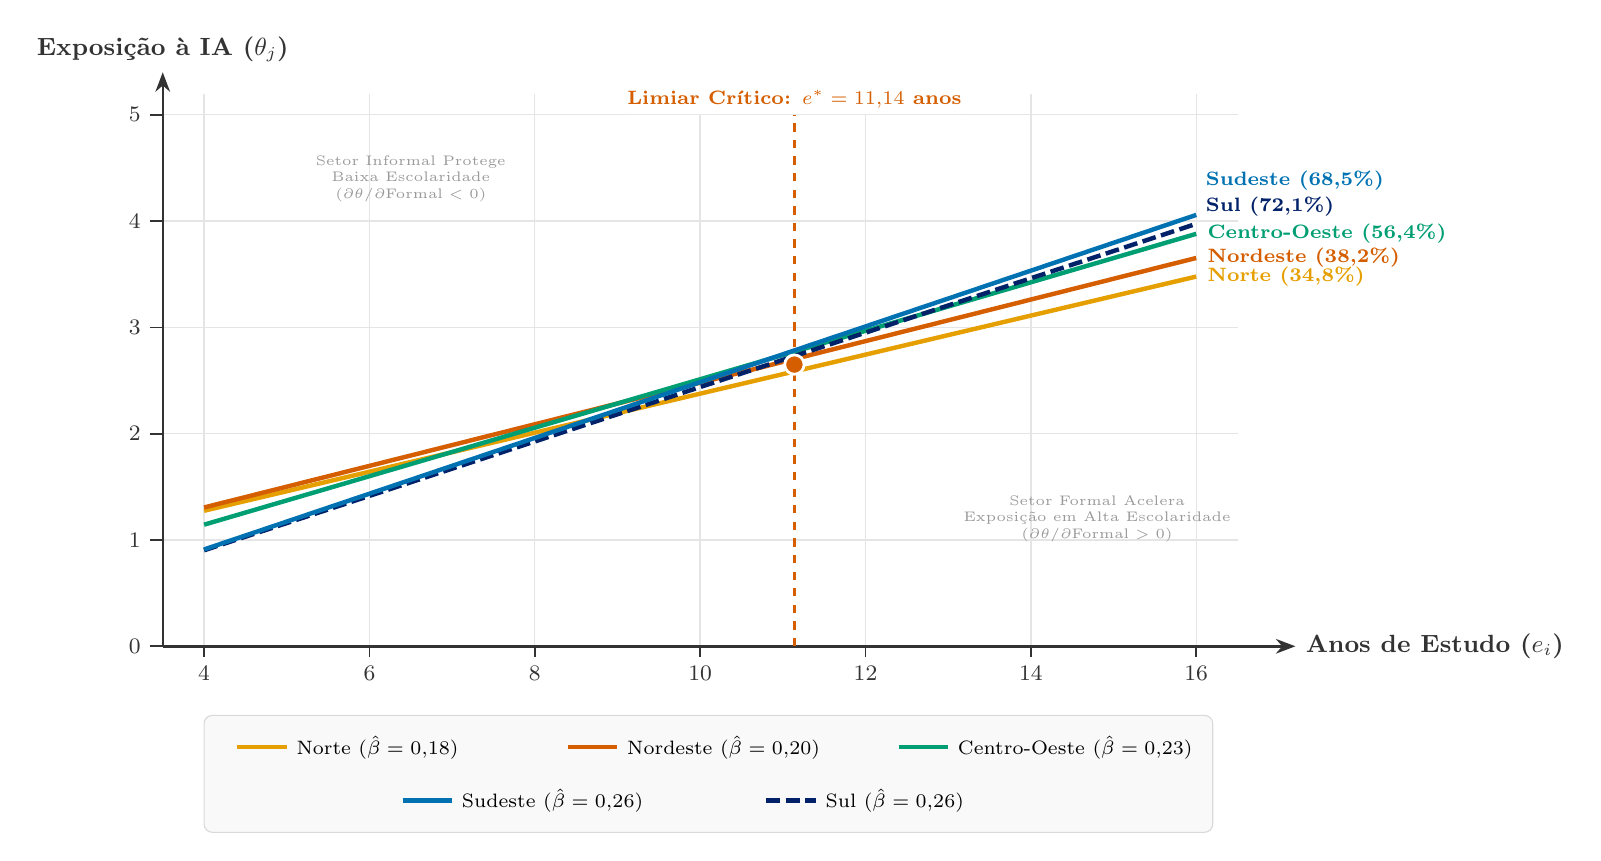
\begin{tikzpicture}[x=1.05cm, y=1.35cm]

  % Background grid lines
  \foreach \x in {4, 6, 8, 10, 12, 14, 16} {
    \draw[gridgray, line width=0.5pt] (\x - 3, 0) -- (\x - 3, 5.2);
    \draw[axisgray, line width=0.6pt] (\x - 3, 0) -- (\x - 3, -0.1);
    \node[below, font=\footnotesize, text=axisgray] at (\x - 3, -0.1) {\x};
  }

  \foreach \y in {0, 1, 2, 3, 4, 5} {
    \draw[gridgray, line width=0.5pt] (0.5, \y) -- (13.5, \y);
    \draw[axisgray, line width=0.6pt] (0.5, \y) -- (0.35, \y);
    \node[left, font=\footnotesize, text=axisgray] at (0.35, \y) {\y};
  }

  % Axes
  \draw[axisgray, line width=0.9pt, ->, >=Stealth] (0.5, 0) -- (14.2, 0) node[right, font=\small\bfseries, text=axisgray] {Anos de Estudo ($e_i$)};
  \draw[axisgray, line width=0.9pt, ->, >=Stealth] (0.5, 0) -- (0.5, 5.4) node[above, font=\small\bfseries, text=axisgray] {Exposição à IA ($\theta_j$)};

  % Threshold e* = 11.14 (X = 11.14 - 3 = 8.14)
  \draw[vermillion, dashed, line width=1.1pt] (8.14, 0) -- (8.14, 5.0);
  \node[above, font=\scriptsize\bfseries, text=vermillion, fill=white, inner sep=2pt, rounded corners=2pt] at (8.14, 5.0) {Limiar Crítico: $e^* = 11{,}14$ anos};

  % Shaded explanatory notes
  \node[font=\tiny, text=gray!80, align=center] at (3.5, 4.4) {Setor Informal Protege\\Baixa Escolaridade\\($\partial \theta / \partial \text{Formal} < 0$)};
  \node[font=\tiny, text=gray!80, align=center] at (11.8, 1.2) {Setor Formal Acelera\\Exposição em Alta Escolaridade\\($\partial \theta / \partial \text{Formal} > 0$)};

  % Regression Lines:
  % Norte: y = 0.5402 + 0.1836 x -> x=4: y=1.275; x=16: y=3.478
  \draw[orange, line width=1.6pt] (4-3, 1.275) -- (16-3, 3.478) node[right, font=\scriptsize\bfseries, text=orange] {Norte (34,8\%)};

  % Nordeste: y = 0.5238 + 0.1956 x -> x=4: y=1.306; x=16: y=3.653
  \draw[vermillion, line width=1.6pt] (4-3, 1.306) -- (16-3, 3.653) node[right, font=\scriptsize\bfseries, text=vermillion] {Nordeste (38,2\%)};

  % Centro-Oeste: y = 0.2320 + 0.2280 x -> x=4: y=1.144; x=16: y=3.880
  \draw[green, line width=1.6pt] (4-3, 1.144) -- (16-3, 3.880) node[right, font=\scriptsize\bfseries, text=green] {Centro-Oeste (56,4\%)};

  % Sul: y = -0.1203 + 0.2559 x -> x=4: y=0.903; x=16: y=3.974
  \draw[instblue, line width=1.6pt, dash pattern=on 5pt off 2pt] (4-3, 0.903) -- (16-3, 3.974);
  \node[right, font=\scriptsize\bfseries, text=instblue] at (13, 4.14) {Sul (72,1\%)};

  % Sudeste: y = -0.1386 + 0.2623 x -> x=4: y=0.911; x=16: y=4.058
  \draw[oitoblue, line width=1.6pt] (4-3, 0.911) -- (16-3, 4.058);
  \node[right, font=\scriptsize\bfseries, text=oitoblue] at (13, 4.38) {Sudeste (68,5\%)};

  % Threshold intersection point (e* = 11.14, y ~ 2.65) -> X = 8.14, Y = 2.65
  \filldraw[fill=vermillion, draw=white, line width=1pt] (8.14, 2.65) circle (3.5pt);

  % Legend box at bottom (2 rows, clean spacing)
  \begin{scope}[shift={(1.0, -1.1)}]
    \draw[draw=gray!30, fill=gray!5, rounded corners=3pt] (0, -0.65) rectangle (12.2, 0.45);
    
    % Row 1
    \draw[orange, line width=1.5pt] (0.4, 0.15) -- (1.0, 0.15);
    \node[right, font=\scriptsize] at (1.0, 0.15) {Norte ($\hat{\beta}=0{,}18$)};

    \draw[vermillion, line width=1.5pt] (4.4, 0.15) -- (5.0, 0.15);
    \node[right, font=\scriptsize] at (5.0, 0.15) {Nordeste ($\hat{\beta}=0{,}20$)};

    \draw[green, line width=1.5pt] (8.4, 0.15) -- (9.0, 0.15);
    \node[right, font=\scriptsize] at (9.0, 0.15) {Centro-Oeste ($\hat{\beta}=0{,}23$)};

    % Row 2
    \draw[oitoblue, line width=1.5pt] (2.4, -0.35) -- (3.0, -0.35);
    \node[right, font=\scriptsize] at (3.0, -0.35) {Sudeste ($\hat{\beta}=0{,}26$)};

    \draw[instblue, line width=1.5pt, dash pattern=on 5pt off 2pt] (6.8, -0.35) -- (7.4, -0.35);
    \node[right, font=\scriptsize] at (7.4, -0.35) {Sul ($\hat{\beta}=0{,}26$)};
  \end{scope}

\end{tikzpicture}
\end{document}
